\documentclass[a4paper,11pt]{article}
\usepackage[T2A]{fontenc}
\usepackage[utf8]{inputenc}
\usepackage[english,russian]{babel}
\usepackage{circuitikz}
\usepackage{wrapfig}
\usepackage{makecell}
\usepackage{tabularx}
\usepackage{graphicx}
\usepackage{gensymb}
\usepackage{cancel} %cancel symbol
\usepackage{amsmath,amsfonts,amssymb,amsthm,mathtools}
\usepackage{pgfplots}
\usepackage[margin=3cm]{geometry}
\pgfplotsset{compat=1.12}
\usepackage{mathrsfs}
\usepackage{multirow}
\usepackage[table,xcdraw]{xcolor}
\usepackage{tabto}
%tikz (draw)

\usepackage{tikz}
\usepackage{pstricks-add}
%tikz libraries

\usetikzlibrary{intersections}
\usetikzlibrary{arrows.meta}
\usetikzlibrary{calc,angles,positioning}
\usetikzlibrary{arrows}
\usepackage{float}

\parindent=0ex % красная строка (ее отсутсвие)

\graphicspath{ {C:/Users/Admin/Documents/TEX/test} }


\begin{document}
    \begin{center}
        МОСКОВСКИЙ ГОСУДАРСТВЕННЫЙ УНИВЕРСИТЕТ \\
        ИМ. М.В. ЛОМОНОСОВА \\
        
        
        \hfill \break
        Факультет вычислительной математики и кибернетики\\
        \vspace{2.5cm}
        \Large{\textbf{Отчет по заданию № 1}}\\
        \vspace{0.5cm}
        \large{\textbf{<<Методы сортировки>>}}\\
        \vspace{0.5cm}
        \large{\textbf{Вариант 3 3 2 4}}\\
        \hfill \break
        \\
    \end{center}
    \begin{flushright}
        \textbf{Исполнитель:}\\ 
        Студент гр. 106\\
        Кондрашов Даниил Сергеевич\\
        \vspace{0.2 cm}
        \textbf{Преподаватели:}\\ 
        Корухова Людмила Сергеевна\\ 
        Манушин Дмитрий Валерьевич \\

    \end{flushright}
    \vfill

    \begin{center}
        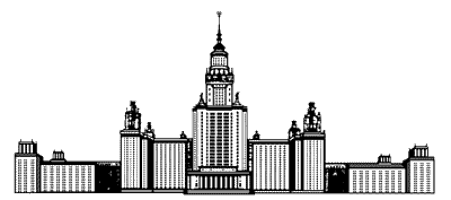
\includegraphics[width = 0.5\linewidth] {msu_logo}
    \end{center}
    \begin{center} 
        Москва, 2024 
    \end{center}
	\thispagestyle{empty} %отсутсвие нумерации на странице

    \newpage
    \tableofcontents %оглавление

    \thispagestyle{empty} %отсутсвие нумерации на странице

    \newpage
    \pagenumbering{arabic} % тип последующей нумерации 
    \section{Постановка задачи}
    \vspace{0,5cm}
    

    \begin{enumerate}
        \item Требуется реализовать два метода сортировки одномерного массива чисел типа \textit{double} (элементы упорядочиваются по неубыванию модулей):\\
        \hspace*{1 cm} 1 -- Сортировка методом простого выбора \\
        \hspace*{1 cm} 2 -- Быстрая сортировка, основанная на рекурсивной реализации
        \item Провести их экспериментальное сравнение, и при реализации каждого метода вычислить число сравнений элементов и число перемещений, занести результаты в таблицу, посчитать среднее, основываясь на трех случаях заполнения массивов:\\
        \hspace*{1.2 cm} 1 -- элементы упорядочены, \\ 
        \hspace*{1.2 cm} 2 -- элементы упорядочены в обратном порядке,\\ 
        \hspace*{1.2 cm} 3 -- расстановка элементов случайна\\
        \vspace{0 cm}\\
        \textit{(\textbf{4 массив был убран из-за ненадобности, потому что каждое значение в таблице - это среднее значение, полученное после 10000 прогонов различных массивов одной длины, именно с этим связано появление дробных чисел в таблице})}
        \item Сравнить асимптотическую сложность алгоритмов. 
        \item На основе полученных результатов сделать вывод.
    \end{enumerate}
    \begin{table}[H]
        \begin{tabular}{|c|c|l|l|l|l|}
        \hline
        \textit{\textbf{Кол-во элементов}}                    & \textbf{Номер сортировки} & \multicolumn{1}{c|}{\textbf{1}} & \multicolumn{1}{c|}{\textbf{2}} & \multicolumn{1}{c|}{\textbf{3}} & \multicolumn{1}{c|}{\textbf{Среднее значение}} \\ \hline
        {\color[HTML]{3F3B42} }                               & Сравнения                 &                                 &                                 &                                 &                                                \\ \cline{2-6} 
        \multirow{-2}{*}{{\color[HTML]{3F3B42} \textbf{10}}}  & Перемещения               &                                 &                                 &                                 &                                                \\ \hline
        {\color[HTML]{3F3B42} }                               & Сравнения                 &                                 &                                 &                                 &                                                \\ \cline{2-6} 
        \multirow{-2}{*}{{\color[HTML]{3F3B42} \textbf{...}}} & Перемещения               &                                 &                                 &                                 &                                                \\ \hline
        \end{tabular}
    \end{table}

    \newpage
    \section{Результаты экспериментов}
    \vspace{0.3cm}
    В результате проведенных экспериментов была подтверждена асимптотическая сложность алгоритмов:
    $O(n^2)$ для сортировки выбором и $O(n\cdot\log_2n)$ для быстрой сорттировки. 

    %\begin{center}
    \hspace{6 cm}\textbf{\Large{Selection sort}}
    %\end{center}
    \vspace{0cm}
    \begin{table}[H]
        \begin{tabular}{|c|c|c|c|c|c|}
        \hline
        \textit{\textbf{N}}                                     & \textbf{Номер сортировки} & \textbf{1}   & \textbf{2}   & \textbf{3}   & \textbf{Среднее значение} \\ \hline
        {\color[HTML]{3F3B42} }                                 & Сравнения                 & 45,0         & 45,0         & 45,0         & 45,0                      \\ \cline{2-6} 
        \multirow{-2}{*}{{\color[HTML]{3F3B42} \textbf{10}}}    & Перемещения               & 6,8          & 6,8          & 7,0          & 6,9                       \\ \hline
        {\color[HTML]{3F3B42} }                                 & Сравнения                 & 1 225,0      & 1 225,0      & 1 225,0      & 1 225,0                   \\ \cline{2-6} 
        \multirow{-2}{*}{{\color[HTML]{3F3B42} \textbf{50}}}    & Перемещения               & 45,5         & 45,2         & 45,7         & 45,4                      \\ \hline
        {\color[HTML]{3F3B42} }                                 & Сравнения                 & 4 950,0      & 4 950,0      & 4 950,0      & 4 950,0                   \\ \cline{2-6} 
        \multirow{-2}{*}{{\color[HTML]{3F3B42} \textbf{100}}}   & Перемещения               & 94,9         & 94,6         & 94,5         & 94,7                      \\ \hline
        {\color[HTML]{3F3B42} }                                 & Сравнения                 & 124 750,0    & 124 750,0    & 124 750,0    & 124 750,0                 \\ \cline{2-6} 
        \multirow{-2}{*}{{\color[HTML]{3F3B42} \textbf{500}}}   & Перемещения               & 492,4        & 493,1        & 493,7        & 493,1                     \\ \hline
        {\color[HTML]{3F3B42} }                                 & Сравнения                 & 499 500,0    & 499 500,0    & 499 500,0    & 499 500,0                 \\ \cline{2-6} 
        \multirow{-2}{*}{{\color[HTML]{3F3B42} \textbf{1000}}}  & Перемещения               & 992,1        & 992,4        & 992,3        & 992,3                     \\ \hline
        {\color[HTML]{3F3B42} }                                 & Сравнения                 & 12 497 500,0 & 12 497 500,0 & 12 497 500,0 & 12 497 500,0              \\ \cline{2-6} 
        \multirow{-2}{*}{{\color[HTML]{3F3B42} \textbf{5000}}}  & Перемещения               & 4 990,4      & 4 990,4      & 4 991,2      & 4 990,7                   \\ \hline
        {\color[HTML]{3F3B42} }                                 & Сравнения                 & 49 995 000,0 & 49 995 000,0 & 49 995 000,0 & 49 995 000,0              \\ \cline{2-6} 
        \multirow{-2}{*}{{\color[HTML]{3F3B42} \textbf{10000}}} & Перемещения               & 9 989,1      & 9 989,6      & 9 990,6      & 9 989,8                   \\ \hline
        \end{tabular}
    \end{table}
    %\begin{center}
    \hspace{6,5 cm}\textbf{\Large{Quick sort }}
    %\end{center}
    \begin{table}[H]
        \begin{tabular}{|c|c|c|c|c|c|}
        \hline
        \textit{\textbf{N}}                                     & \textbf{Номер сортировки} & \textbf{1} & \textbf{2} & \textbf{3} & \textbf{Среднее значение} \\ \hline
        {\color[HTML]{3F3B42} }                                 & Сравнения                 & 50.3       & 50.7       & 47.8       & 49.6                      \\ \cline{2-6} 
        \multirow{-2}{*}{{\color[HTML]{3F3B42} \textbf{10}}}    & Перемещения               & 12.8       & 12.9       & 13.4       & 13.0                      \\ \hline
        {\color[HTML]{3F3B42} }                                 & Сравнения                 & 523.4      & 514.9      & 398.2      & 478.8                     \\ \cline{2-6} 
        \multirow{-2}{*}{{\color[HTML]{3F3B42} \textbf{50}}}    & Перемещения               & 90.0       & 89.8       & 93.9       & 91.2                      \\ \hline
        {\color[HTML]{3F3B42} }                                 & Сравнения                 & 1293.0     & 1328.5     & 912.8      & 1178.1                    \\ \cline{2-6} 
        \multirow{-2}{*}{{\color[HTML]{3F3B42} \textbf{100}}}   & Перемещения               & 202.1      & 200.7      & 211.3      & 204.7                     \\ \hline
        {\color[HTML]{3F3B42} }                                 & Сравнения                 & 12972.5    & 13215.3    & 6278.6     & 10822.1                   \\ \cline{2-6} 
        \multirow{-2}{*}{{\color[HTML]{3F3B42} \textbf{500}}}   & Перемещения               & 1215.5     & 1212.2     & 1334.1     & 1253.9                    \\ \hline
        {\color[HTML]{3F3B42} }                                 & Сравнения                 & 32118.6    & 31994.0    & 13939.0    & 26017.2                   \\ \cline{2-6} 
        \multirow{-2}{*}{{\color[HTML]{3F3B42} \textbf{1000}}}  & Перемещения               & 2605.0     & 2607.1     & 2893.0     & 2701.7                    \\ \hline
        {\color[HTML]{3F3B42} }                                 & Сравнения                 & 291617.3   & 306776.7   & 85866.4    & 228086.8                  \\ \cline{2-6} 
        \multirow{-2}{*}{{\color[HTML]{3F3B42} \textbf{5000}}}  & Перемещения               & 15159.5    & 15144.3    & 17223.3    & 15842.4                   \\ \hline
        {\color[HTML]{3F3B42} }                                 & Сравнения                 & 819394.8   & 828068.8   & 185012.2   & 610825.2                  \\ \cline{2-6} 
        \multirow{-2}{*}{{\color[HTML]{3F3B42} \textbf{10000}}} & Перемещения               & 32316.7    & 32028.3    & 36936.6    & 33760.5                   \\ \hline
        \end{tabular}
    \end{table}
    * количество массивов было сокоращено с 4 до 3, потому что каждое значение в таблице это средний результат из 10000 прогонов различных массивов одной длины\\

    \large{\textbf{Вывод:}} 
    В результате проведеных опытов были подтверждены формулы, использующиеся для нахождения асимптотической сложности алгоритмов, и было сделано заключение о том, что quick sort быстрее, чем selection sort, но для этого нужны наиболее случайные значения, при росте количества элементов массива эта разница становится заметнее еще больше.


    \newpage
    \section{Структура программы и спецификация функций}
    \vspace{0,5cm}
    Для более оптимизированной работы программы использовались функции, которые работали как с массивом данных, так и с численными перменными.
    \vspace{0.9cm}\\
    \textbf{Список функций:}\\
    \begin{enumerate}
        \item change() -- функция меняет местами два элемента массивов, которые ей подаются.
        \item selection\_sort() -- функция сортирует массив методом выбора и подсчитывает количество изменений и сравнений, которые были при этом сделаны.
        \item fast\_sort() -- функция сортирует массив методом быстрой сортировки рекурсией и подсчитывает количество изменений и сравнений, которые были при этом сделаны.
        \item sort\_q() -- сортирует массив по возрастанию, используя алгоритм selection sort.
        \item sort\_rev() -- сортирует массив в обратнмо порядке, используя алгоритм selection sort.
        \item filling() -- заполняет массив случайным числами, используя условие, которое было выбрано.
        \item sred() -- подсчитывает среднее из всех элементов массива
    \end{enumerate}
    \newpage
    \section{Отладка программы, тестирование программы}
    \vspace{0,5cm}
    Для проверки корректности сортировки, перед выводом результатов, массивы, полученные после выполнения функций, проверялись на упорядоченность. В случае неправильного расположения  элементов, в консоль выводилось сообщение об ошибке.\\
    Для отладки и соотвествующей тестировки программы в каждую из сортирующий функций был добавлен вывод массива после каждого прохода по нему.\\ 
    \vspace{0.2 cm}\\
    Далее представлены примеры прохода по \textbf{случайным} массивам и их сортировка нашими функциями\\
    
    \textbf{selection\_sort} \\
    \textit{изначально функции подается неупорядоченный массив из 7 элементов, после 5 проходов возвращается упорядоченный массив}\\
    \vspace{0.1cm}\\
    172.00\qquad 5992.90\qquad -4900.79\qquad -7914.01\qquad 24101.29\qquad 5888.81\qquad 
    -12516.97\qquad \\
    172.00\qquad -4900.79\qquad 5992.90\qquad -7914.01\qquad 24101.29\qquad 5888.81\qquad 
    -12516.97\qquad \\
    172.00\qquad -4900.79\qquad 5888.81\qquad -7914.01\qquad 24101.29\qquad 5992.90\qquad 
    -12516.97\qquad \\
    172.00\qquad -4900.79\qquad 5888.81\qquad 5992.90\qquad 24101.29\qquad -7914.01\qquad 
    -12516.97\qquad \\
    172.00\qquad -4900.79\qquad 5888.81\qquad 5992.90\qquad -7914.01\qquad 24101.29\qquad 
    -12516.97\qquad \\
    172.00\qquad -4900.79\qquad 5888.81\qquad 5992.90\qquad -7914.01\qquad -12516.97\qquad 24101.29\qquad \\
    
    \vspace{0.1cm}
    \textbf{quick\_sort} \\
    \textit{изначально функции подается неупорядоченный массив из 7 элементов, и возвращается массив, упорядоченный согласно нашему условию.}\\ 
    \textbf{|} \textit {- показывает разбиение на подмассивы с которыми работает рекурсивная функция}\\
    \vspace{0.1cm}\\
    172.00\qquad 5992.90\qquad -4900.79\qquad 5888.81\qquad 24101.29\qquad -7914.01\qquad -12516.97\qquad \\ 
    172.00\qquad -4900.79\qquad 5992.90\qquad 5888.81\quad | \quad-7914.01\qquad 24101.29\qquad -12516.97\qquad \\ 
    172.00\qquad -4900.79\quad | \enspace5888.81\qquad5992.90\quad|\quad-7914.01\quad|\quad-12516.97 \quad24101.29\qquad \\ 
    
    \vspace{0.5cm}
    \small{P.S. при проверке отсортированного массива не стоит забывать, что элементы сортируются по неубыванию модулей}

    \newpage
    \section{Анализ допущенных ошибок}
    \vspace{0,5cm}
    При написании функции 
    \textbf{fast\_sort()} для сортировки массива методом быстрой сортировки (рекурсивная реализация), была допущена ошибка: \\
    значение pivot (опорного элемента) сохранялось, как значение индекса этого элемента в массиве, а не как вещественное число, из-за чего при выполнение функции значение pivot могло меняться в течение одного прохода, что привело к неправильной сортировке массивов.   


    \newpage
    \section{Литература}
    \vspace{0.5cm}

    \begin{thebibliography}{10}
        \vspace{0.5cm}
        \bibitem{}
        Трифонов Н. П., Пильщиков В. Н. Задания практикума на ЭВМ (1 курс). Методическая разработка(составители). — М.: ВМК МГУ, 2001.
        \bibitem{}
        Кормен Т., Лейзерсон Ч., Ривест Р., Штайн К. Алгоритмы: построение и анализ. Второе издание.
        — М.: «Вильямс», 2005.
        \bibitem{}
        Головинов Г.  Основы программирования на TeX. Том 1. Начало. — М.: МФТИ, 2024.
        \bibitem{}
        Кнут Д. Искусство программирования для ЭВМ. Том 3. — М.: Мир, 1978.
        \bibitem{}
        Лорин Г. Сортировка и системы сортировки. — М.: Наука, 1983.
    \end{thebibliography}

    


\end{document}

